% vqa.tex

% vqa structure


\begin{frame}
    \frametitle{Variational Quantum Algorithms}

    Variational Quantum Algorithms (VQA) form the idea of using a proposed
    architecture for generalised learning problems on NISQ systems
    \cite{bharti2021noisy}.

    \begin{figure}
        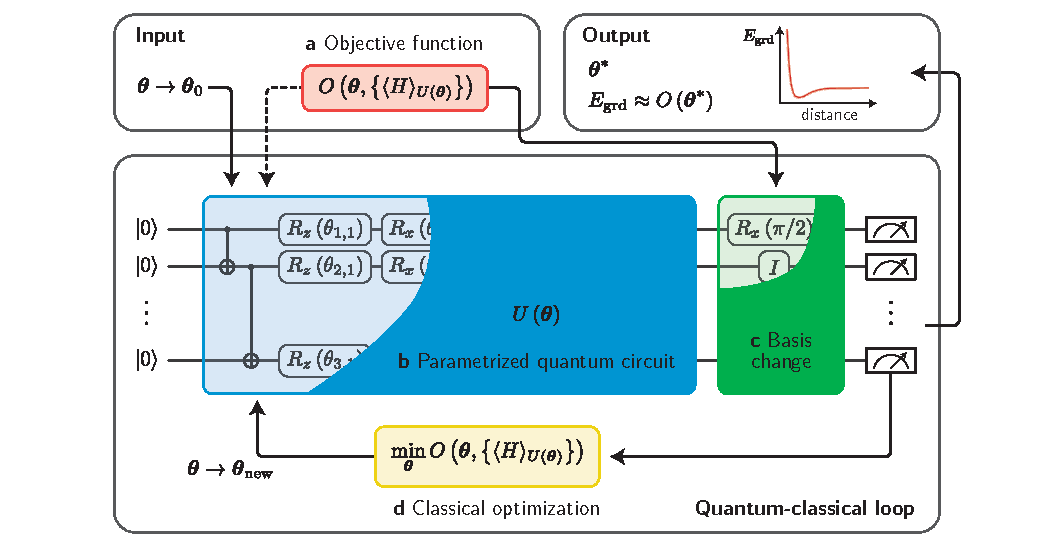
\includegraphics[width=0.8\textwidth]{figures/vqaarch.pdf}
    \end{figure}
\end{frame}

% where does this slot in?

\begin{frame}
    \frametitle{Transitioning}

    \begin{figure}
        \centering
        
        \begin{subfigure}{0.45\textwidth}
            \centering
            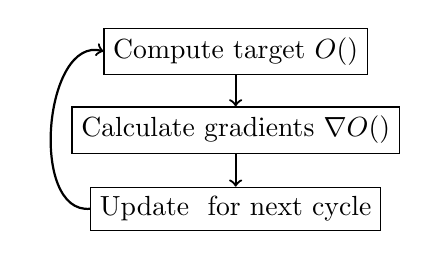
\begin{tikzpicture}[every node/.style=draw,rectangle] 
                \node (opt) [] {Compute target \(O(\vecx)\)};
                \node (grad)[below of=opt] {Calculate gradients \(\nabla O(\vecx)\)};
                \node (upd) [below of=grad] {Update \(\vecx\) for next cycle};

                \draw[->, thick] (opt) to (grad);
                \draw[->, thick] (grad) to (upd);
                \draw[->, thick, bend left=100] (upd.west) to (opt.west);
            \end{tikzpicture}
        \end{subfigure}
        %
        \begin{subfigure}{0.45\textwidth}
            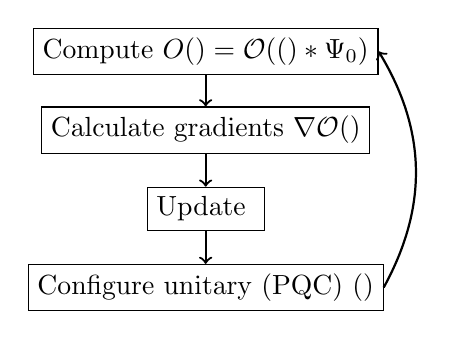
\begin{tikzpicture}[every node/.style=draw,rectangle] 
                \node (opt) [] {Compute \(O(\parameters) = \mathcal{O}(\pqc(\parameters)\ket*{\Psi_0})\)};
                \node (grad)[below of=opt] {Calculate gradients \(\nabla \mathcal{O}(\parameters)\)};
                \node (uni)[below of=grad] {Update \(\parameters\)};
                \node (upd) [below of=uni] {Configure unitary (PQC) \(\pqc(\parameters)\)};
    
                \draw[->, thick] (opt) to (grad);
                \draw[->, thick] (grad) to (uni);
                \draw[->, thick] (uni) to (upd);
                \draw[->, thick, bend right] (upd.east) to (opt.east);
            \end{tikzpicture}
        \end{subfigure}
    \end{figure}

    \begin{center}
        \(\parameters \in \reals^M, \vecx \in \reals^N, M \sim \lceil{\log_2 N}\rceil\)
    \end{center}

\end{frame}

% detailed look at PQCs
% dla
\begin{frame}
    \frametitle{Parametrized Quantum Circuits (PQCs)}

    The actual unitary computation happens in an L-layered structure with the
    mathematical form

    \begin{gather}
        \pqc(\parameters) = \prod\limits_{l = 1}^{L} U_l(\parameters_l), \quad
        \pqc_l(\parameters) = \prod\limits_{k = 1}^{K} e^{-\iota \theta_{lk} H_k}~.
        \label{eq:pqc}
    \end{gather}

    for a set of generators \(\{H_k\}\) with \(\parameters = (\parameters_1,
    \parameters_2, \ldots, \parameters_k)\).

    Formally, the generators create a Dynamical Lie Algebra, which determines
    the set of reachable unitaries. The choice of generators can strongly affect
    the optimization process \cite{larocca2021diagnosing}. See the report for a
    detailed study.

\end{frame}

% qlt
\begin{frame}
    \frametitle{Quantum Landscape Theory}

    Spaces and maps involved in VQA calculation \cite{larocca2021theory}:

    \begin{figure}
        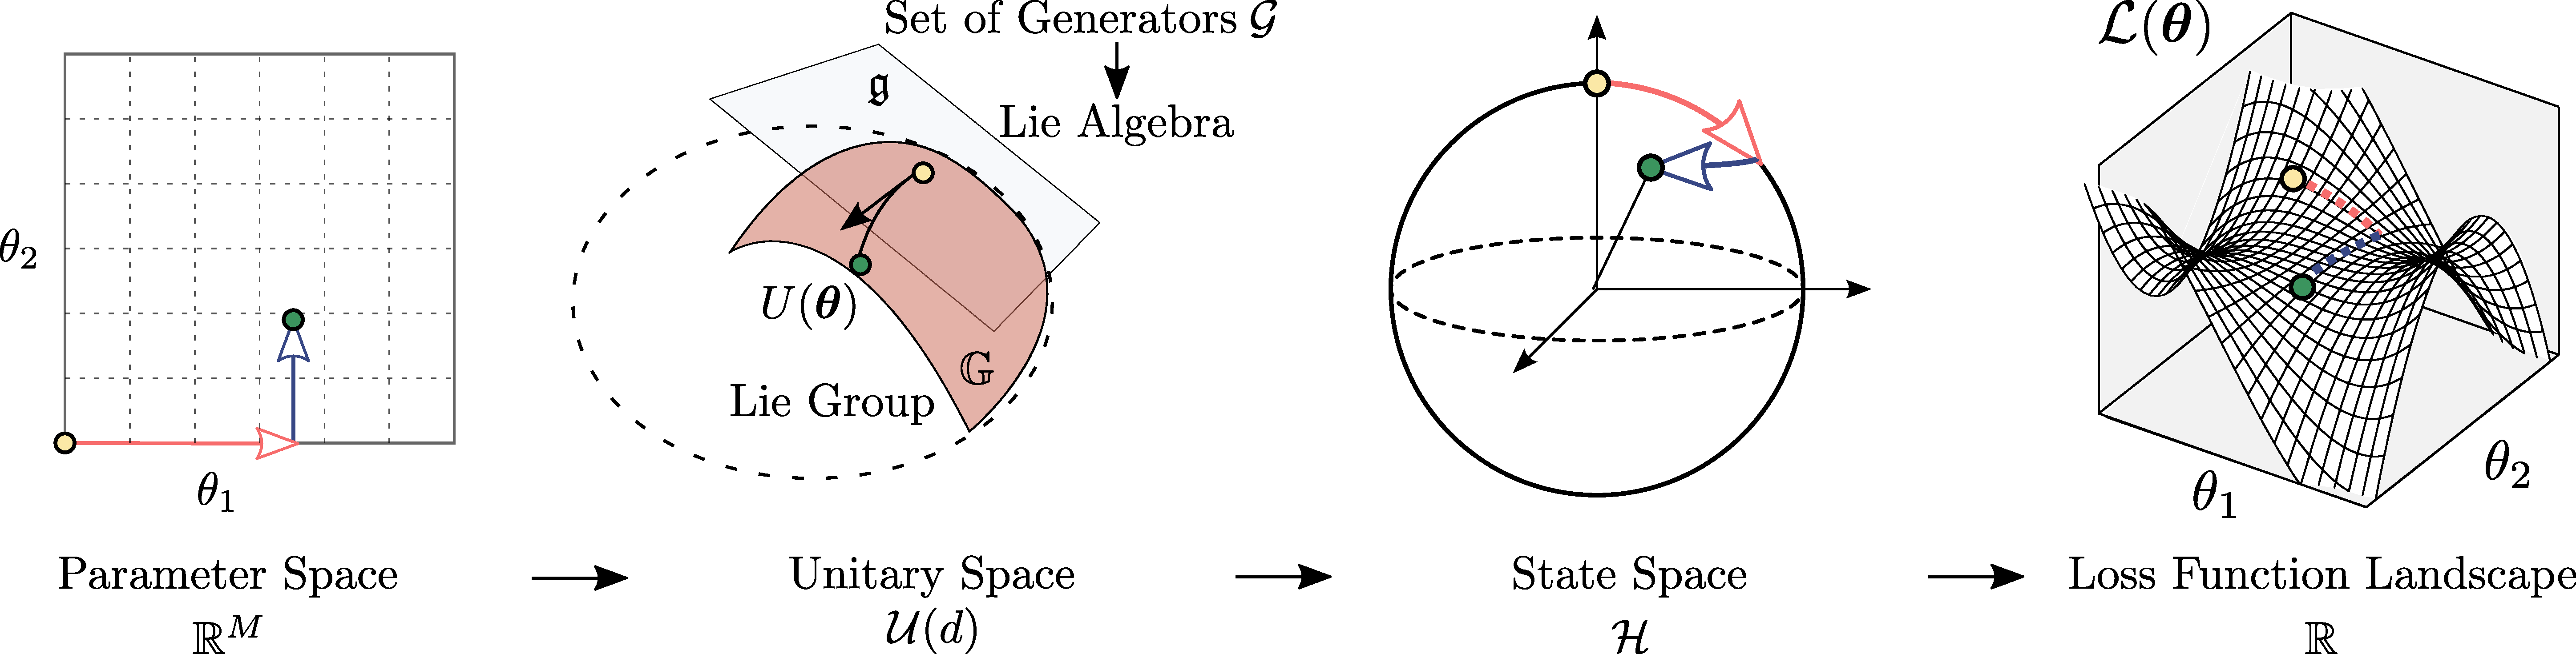
\includegraphics[width=0.8\textwidth]{figures/mapsurjective.pdf}
    \end{figure}

    This structure forms the playground for our analysis. The study of these
    spaces forms an important part of establishing relative bounds at stages of
    the calculation (which are the spaces). We discuss the particular case of
    \(\mathcal{U}(d) \to \hilbertspace\) here. See the report for details on the
    other maps.

\end{frame}
